\section{Below the measure threshold: positive differences settle the zero question}
\label{subpick:sec:main}
The failure of finite signed-moment representability below $a+b=1$
does not imply a failure of positivity after a discrete derivative.
Consecutive differences supply a finite positive measure and resolve
the slit-plane nonvanishing and angular-uniqueness questions left open
by the real-order reports. They also extend the right-endpoint radial
mechanism from the critical line to the entire subcritical region.

Write $c_n=H_{n-1}^{(b)}/n^a$ and $F_{a,b}(z)=\sum_{n\ge1}c_nz^n$.
For $a>0$, $b>0$, $w=a+b<1$, put $s=w-1\in(-1,0)$ and
\begin{align}
 k_v(T)&=T^{v-1}/\Gamma(v),\\
 \mathfrak h(t)&=(1-e^{-t})^{-1}-t^{-1},\\
 \mathcal C_{a,b}(T)&=\frac1{\Gamma(a)\Gamma(b)}
  \int_0^T(T-t)^{a-1}t^{b-1}\mathfrak h(t)\,dt,\\
 R_{a,b}(T)&=-\zeta(b)k_a(T)-\frac{k_s(T)}{1-b}
                +\mathcal C_{a,b}(T).\label{subpick:eq:R}
\end{align}
Here $k_s$ is a signed function, not a positive Gamma density:
$\Gamma(s)=\Gamma(s+1)/s<0$. Since $0<b<1$, $\zeta(b)<0$,
and $1/2<\mathfrak h(t)<1$, all three terms of $R_{a,b}$ are
strictly positive. The regularized Hurwitz identity used here is
\[
 \zeta(b,n)=\frac{n^{1-b}}{b-1}
 +\frac1{\Gamma(b)}\int_0^\infty e^{-nt}t^{b-1}\mathfrak h(t)\,dt;
\]
it follows from the convergent Hurwitz integral by subtraction and
analytic continuation in $b$, as in the preceding construction
\cite{intdist:DLMFHurwitz}.

\begin{theorem}[Positive Hausdorff differences]
\label{subpick:thm:differences}
For $a,b>0$ with $a+b<1$, define
\[
 d\omega_{a,b}(u)=(1-u)R_{a,b}(-\log u)\,du,\qquad 0<u<1.
\]
This is a finite positive measure, with strictly positive density and
mass $2^{-a}$. For every $n\ge1$,
\begin{align}
 c_n&=\int_0^1(1-u^{n-1})R_{a,b}(-\log u)\,du,
       \label{subpick:eq:bernstein}\\
 c_{n+1}-c_n&=\int_0^1u^{n-1}\,d\omega_{a,b}(u).
       \label{subpick:eq:differences}
\end{align}
The first measure has infinite mass, but every displayed integral is
absolutely convergent. Thus the shifted sequence $c_{n+1}$ is a discrete
Bernstein sequence, and its differences are strictly completely monotone.
Here $\Delta f_n=f_{n+1}-f_n$. In particular, for all $j\ge0$ and $n\ge1$,
\[
 (-1)^j\Delta^j(c_{n+1}-c_n)
   =\int_0^1u^{n-1}(1-u)^j\,d\omega_{a,b}(u)>0.
\]
The positive difference measure is uniquely determined by these moments.
\end{theorem}
\begin{proof}
At $T=0$, the leading term of $R$ is a positive constant times
$T^{w-2}$; the other terms have orders $T^{a-1}$ and $T^{w-1}$.
Multiplication by $1-e^{-T}$ therefore makes it integrable, since
$w>0$. At infinity all terms grow at most polynomially and the change
of variables $u=e^{-T}$ supplies $e^{-T}$. This proves finiteness of
$\omega$, convergence of \eqref{subpick:eq:bernstein}, and divergence
of the unweighted mass at $u=1$.

For $s\in(-1,0)$, integration by parts gives the convergent identity
\[
 \int_0^\infty(e^{-T}-e^{-nT})k_s(T)\,dT=1-n^{-s}.
\]
Both boundary terms vanish: near zero their order is $T^{s+1}$,
and infinity has exponential decay. For $k_a$ the same identity is
the ordinary Gamma integral. The convolution has Laplace transform
\[
 \int_0^\infty e^{-nT}\mathcal C_{a,b}(T)\,dT
 =n^{-a}\left(\zeta(b,n)+\frac{n^{1-b}}{1-b}\right).
\]
Every convolution interchange is absolute. Insert these three identities
into \eqref{subpick:eq:R}, with the factor $e^{-T}-e^{-nT}$ retained.
The constant and power terms cancel, leaving
$n^{-a}(\zeta(b)-\zeta(b,n))=c_n$. No divergent Laplace transforms
are subtracted. Subtract the two convergent formulas at $n+1$ and $n$
to obtain \eqref{subpick:eq:differences}. At $n=1$ this gives mass
$c_2=2^{-a}$. The difference formula proves every strict sign, and
polynomial density on $[0,1]$ proves uniqueness of the finite measure.
\end{proof}

On the critical line $a=1-b>0$, use instead
$R_{a,b}=-\zeta(b)k_a+\mathcal C_{a,b}$. Its finite mass is $1/a$,
and its Laplace transform is $1/a-c_n$, so the same formulas for
$\omega=(1-u)R(-\log u)\,du$ hold. This is precisely the negative
density of the critical signed measure; its positive atom at one
disappears after multiplication by $1-u$.
On the whole axis $a=0,b>0$, the difference measure is simply
\[
 d\omega_{0,b}(u)=\frac{(-\log u)^{b-1}}{\Gamma(b)}\,du,
 \qquad c_{n+1}-c_n=n^{-b},
\]
and $F_{0,b}(z)=z\Li_b(z)/(1-z)$. These measures also have strictly
positive densities, with mass $2^{-a}$ and no endpoint atoms.

\begin{corollary}[A sharp complementary positivity classification]
\label{subpick:cor:classification}
For $a\ge0,b>0$, the consecutive differences $c_{n+1}-c_n$ are
moments of a finite positive measure on $[0,1]$ if and only if
$a=0$ or $a+b\le1$. In the same parameter region the function
\[
 \Phi_{a,b}(t)=(t+1)^{-a}
       \{\zeta(b)-\zeta(b,t+1)\},\qquad t\ge0,
\]
with $\gamma+\psi(t+1)$ replacing the braces at $b=1$, is a
Bernstein function: $\Phi(0)=0$, $\Phi(t)>0$ for $t>0$, and
$(-1)^j\Phi^{(j+1)}(t)>0$ for all $j\ge0$.
\end{corollary}
\begin{proof}
The preceding proof works for every real $n\ge1$, since the Gamma
and regularized Hurwitz identities used there do not require integer
$n$. Thus $\Phi(t)=\int(1-u^t)\,d\rho(u)$ with
$d\rho=d\omega/(1-u)$. Differentiation gives
\[
 (-1)^j\Phi^{(j+1)}(t)
   =\int_0^1(-\log u)^{j+1}u^t\,d\rho(u)>0.
\]
All these integrals converge even at $t=0$: the endpoint at one is
controlled by $\int(1-u)\,d\rho<\infty$, and the logarithmic-coordinate
density at zero has exponential decay times polynomial growth.
The same representation follows on the axis from the ordinary Hurwitz
integral, or its convergent difference at $b\le1$.

Conversely, for $a>0,a+b>1$, elementary harmonic asymptotics give
$c_n\to0$ while $c_2=2^{-a}>0$. The sequence cannot be nondecreasing,
so its differences cannot all be positive-measure moments and its
continuous interpolation cannot be a Bernstein function. This proves
both sharp parameter statements.
\end{proof}

\begin{theorem}[Global nonvanishing at all positive inner orders]
\label{subpick:thm:global}
For every $a\ge0$, $b>0$, the principal continuation of $F_{a,b}$
has no zero on $\C\setminus[1,\infty)$ except its double zero at zero.
For $a>0$, $a+b\le1$, and also for $a=0,b>0$, the stronger factorization is
\begin{equation}\label{subpick:eq:factor}
 F_{a,b}(z)=\frac{z^2}{1-z}P_{a,b}(z),\qquad
 P_{a,b}(z)=\int_0^1\frac{d\omega_{a,b}(u)}{1-zu}.
\end{equation}
In particular $P(0)=2^{-a}$, $\Imag P(z)$ has the strict sign of
$\Imag z$, and $P(x)>0$ for every real $x<1$.
\end{theorem}
\begin{proof}
The coefficient of $z^m$ in $(1-z)F(z)/z^2$ is
$c_{m+2}-c_{m+1}$, including $m=0$ because $c_1=0$.
The difference moments give \eqref{subpick:eq:factor} in the disk.
The finite positive measure gives holomorphic continuation to the slit
plane, where its imaginary-part and real-axis signs prove nonvanishing.
The mass proves multiplicity exactly two. For $a>0,a+b>1$, the
one-crossing finite signed measure already gives
$F=z^2P_r/(1-rz)$ with a nonzero positive Stieltjes transform and
$0<r<1$. The same argument applies. This proves the complete parameter
statement while retaining the sharp boundary for finite signed moments.
\end{proof}

\subsection{Angular uniqueness and a full subcritical radial theorem}
\begin{theorem}[Right-endpoint Stieltjes geometry]
\label{subpick:thm:radial}
For $a,b>0$ with $a+b\le1$, and for $a=0,b>0$, every open upper
semicircle of radius $0<\rho\le1$ has exactly one simple zero of
$\Imag F_{a,b}$. Its angle satisfies
\[
 \arccos\rho<\theta_{a,b}(\rho)<\arccos(\rho/2),
 \qquad \tfrac12<\eta_{a,b}(\rho)=\cos\theta_{a,b}(\rho)/\rho<1.
\]
The imaginary part is positive before that angle and negative after it.
The normalized quantity $\eta_{a,b}$ is strictly increasing in $\rho$.
Together with the supercritical angular theorem, this proves angular
uniqueness for every $a\ge0,b>0$, including the formerly conjectural
subcritical region. Boundary values are analytic or Abel values where
the ordinary Fourier series does not converge.
\end{theorem}
\begin{proof}
The following argument works for any finite positive measure $\omega$
with a strictly positive density on $(0,1)$. Set $x=\rho^2$,
$m=2\cos\theta/\rho-1$, and
\[
 D(u)=1+x\{u^2-(1+m)u\},\qquad
 G(m,x)=\int_0^1\frac{m-u}{D(u)}\,d\omega(u).
\]
From \eqref{subpick:eq:factor}, direct rationalization gives
\[
 \Imag F(\rho e^{i\theta})
  =\frac{\rho^3\sin\theta}{|1-\rho e^{i\theta}|^2}G(m,x).
\]
For $0<m<1$ all denominators are positive, and
\[
 G_m=\int_0^1\frac{1-xu}{D(u)^2}\,d\omega(u)>0.
\]
We have $G(0,x)<0$. For $x<1$, $G(1,x)>0$.
At $x=1$, its negative part for $u>m\ge1/2$ is bounded in magnitude
by $2\omega((m,1))$, which tends to zero. Its positive part tends
pointwise to $d\omega(u)/(1-u)$ and has a strictly positive limit
inferior by Fatou's lemma, with infinity allowed. Hence $G(m,1)>0$
for some $m<1$. This proves a unique root in $(0,1)$ even when
$\omega/(1-u)$ has infinite mass. Outside that interval the numerator
has a fixed sign, proving uniqueness on the full upper arc.
At the zero, the angular derivative is
$-2\rho^2\sin^2\theta\,G_m/|1-\rho e^{i\theta}|^2<0$.

At a root, the probability measure proportional to $d\omega/D$ has
mean $m$. For $d(u)=u^2-(1+m)u$, the identities
$d(m)=-m$ and $d(u)-d(m)=(u-m)(u-1)$ give
\[
 G_x=-\frac1{1-xm}\int_0^1
                 \frac{(u-m)^2(1-u)}{D(u)^2}\,d\omega(u)<0.
\]
Consequently
\[
 \frac{dm}{dx}
 =\frac{\displaystyle\int (u-m)^2(1-u)D(u)^{-2}\,d\omega(u)}
 {(1-xm)\displaystyle\int(1-xu)D(u)^{-2}\,d\omega(u)}>0,
 \qquad \eta'(\rho)=\rho m'(\rho^2)>0.
\]
All differentiations are dominated locally at the interior root,
including at $x=1$ since $m<1$. The implicit-function theorem proves
smooth dependence. This argument uses only the finite measure $\omega$;
it does not apply a finite-measure limit theorem to its infinite
unweighted predecessor.
\end{proof}

\subsection{One-sided Euler certificates even for divergent boundary series}
\begin{theorem}[Subcritical Euler continuation and a sharp fixed-pair constant]
\label{subpick:thm:euler}
For the parameters of Theorem~\ref{subpick:thm:radial}, put
$A_k=c_{2k+1}$, $g_{a,b}=\Imag F_{a,b}(i)$ and
\[
 E_N=\sum_{j=0}^{N-1}2^{-j-1}
             \sum_{k=0}^j(-1)^k\binom jk A_k.
\]
Then $E_N$ decreases strictly to the analytic Gaussian value, and
\begin{align}
 -g_{a,b}&=\frac12\int_0^1\frac{1+u}{1+u^2}\,d\omega(u),\\
 E_N-g_{a,b}&=2^{-N}\int_0^1
       \frac{(1+u)(1-u^2)^{N-1}}{1+u^2}\,d\omega(u)>0.
       \label{subpick:eq:euler-tail}
\end{align}
The least constant in $E_N-g\le C2^{-N}$ for all $N\ge1$ is
$C=-2g$, and
\[
 2^{-a}<-2g_{a,b}<\frac{1+\sqrt2}{2}\,2^{-a}<\frac54.
\]
Thus $E_N-(5/4)2^{-N}<g_{a,b}<E_N$ is a rational enclosure throughout
this domain. It concerns analytic continuation when the ordinary
alternating series diverges.
\end{theorem}
\begin{proof}
For $j\ge1$, the finite binomial difference of $A_k$ is
\[
 -\int_0^1(1+u)(1-u^2)^{j-1}\,d\omega(u),
\]
while the order-zero difference is $A_0=0$. Sum the geometric tail
against the finite measure to get \eqref{subpick:eq:euler-tail}.
Evaluating \eqref{subpick:eq:factor} at $i$ gives the same limiting
value. The scaled errors decrease strictly to zero, and their largest
value is $2(E_1-g)=-2g$. Finally $(1+u)/(1+u^2)$ has minimum one
at the endpoints and maximum $(1+\sqrt2)/2$ at $u=\sqrt2-1$.
The positive density makes both bounds strict, and the measure has
mass $2^{-a}$. Since $\sqrt2<3/2$, the rational bound follows.
\end{proof}

The global integer-outer-order normalized-radius conjecture remains open.
The new radial theorem covers the full subcritical and critical region
and the zero outer-order axis; it does not assert the same radial
direction in the supercritical region, where fractional turning points
are possible. Finite signed-moment existence, analytic nonvanishing,
angular uniqueness and radial motion now have explicitly different scopes.

\begin{corollary}[An exact Gaussian identity on the outer-order axis]
\label{subpick:cor:axis}
For every $b>0$, with analytic or Abel interpretation when necessary,
\[
 g_{0,b}=-\frac12\left(\beta(b)+2^{-b}\eta(b)\right),
 \qquad \eta(b)=\sum_{n\ge1}\frac{(-1)^{n-1}}{n^b}.
\]
In particular $g_{0,1}=-\pi/8-\log2/4$ and
$g_{0,2}=-G/2-\pi^2/96$.
\end{corollary}
\begin{proof}
The defining residue classes give
$\Li_b(i)=-2^{-b}\eta(b)+i\beta(b)$. Since
$F_{0,b}(i)=i\Li_b(i)/(1-i)=(-1+i)\Li_b(i)/2$,
its imaginary part is the claimed expression. Both Dirichlet series
converge for $b>0$; the depth-two series retains its stated boundary
interpretation. These formulas also identify the sharp fixed-pair
Euler constant as $\beta(b)+2^{-b}\eta(b)$ on this axis.
\end{proof}

\begin{theorem}[Strict Gaussian decrease in the real outer order]
\label{subpick:thm:Gaussian-order}
For every fixed $b>0$, the positive magnitude $-g_{a,b}$ decreases
strictly as $a$ runs through $[0,\infty)$. In particular, for $a>0$,
\[
 0<-2g_{a,b}<\beta(b)+2^{-b}\eta(b)<\frac{1+\sqrt2}{2}.
\]
The supremum over nonnegative outer orders is the explicit axis value.
This is a magnitude bound; it is not an Euler remainder constant in
parameter regions where the right-endpoint Stieltjes factorization
does not apply.
\end{theorem}
\begin{proof}
The outer Gamma integral, first by coefficient comparison in the disk
and then by locally dominated continuation to the slit plane, is
\[
 F_{a,b}(z)=\frac1{\Gamma(a)}\int_0^\infty
                      t^{a-1}F_{0,b}(ze^{-t})\,dt\qquad(a>0).
\]
Near zero its boundary value at $z=i$ is bounded; at infinity the
integrand without $t^{a-1}$ is $O(e^{-2t})$. Let
$h_b(t)=e^t[-\Imag F_{0,b}(ie^{-t})]$. The positive axis measure gives,
with $\rho=e^{-t}$,
\[
 h_b(t)=\int_0^1
  \frac{(1+u)\rho^2}{(1+\rho^2)(1+u^2\rho^2)}\,d\omega_{0,b}(u).
\]
The derivative in $\rho$ of the displayed kernel is
\[
 \frac{2\rho(1+u)(1-u^2\rho^4)}
 {(1+\rho^2)^2(1+u^2\rho^2)^2}>0\qquad(0<\rho\le1,\ 0<u<1).
\]
Thus $h_b$ is positive, bounded and strictly decreasing in $t$.
The Gamma integral is equivalently
$-g_{a,b}=\mathbb E[h_b(T_a)]$, where $T_a\sim\mathrm{Gamma}(a,1)$.
Independent Gamma variables satisfy $T_{a+d}\overset{d}=T_a+T_d$;
strict decrease of $h_b$ proves strict decrease of the expectation.
At $a=0$ take $T_0=0$, and bounded continuity gives the same strict
comparison and the limit as $a\downarrow0$.
For $a>0$, differentiation also gives the exact negative covariance
$\partial_a(-g_{a,b})=\Cov(\log T_a,h_b(T_a))<0$.
The axis identity and its positive-measure bound complete the proof.
\end{proof}

\begin{theorem}[Gaussian monotonicity at every fixed total order]
\label{subpick:thm:fixed-total}
For every $w>0$, $a\mapsto-2g_{a,w-a}$ decreases strictly on $(0,w)$.
Its endpoint limits give the exact strict inequalities
\[
 2\{\beta(w)-\beta(w-1)\}
 <-2g_{a,w-a}<\beta(w)+2^{-w}\eta(w).
\]
Here $\beta(w-1)$ uses analytic continuation when necessary.
In particular, this proves the previously conjectural strict decrease
on the entire critical line $w=1$.
\end{theorem}
\begin{proof}
In the positive double kernel put $x=e^{-s}$, $y=e^{-(s+t)}$,
then $T=s+t$ and $R=s/T$. Its Gaussian value becomes
\[
 -g_{a,b}=\mathbb E[K(R,T)],\qquad
 K(R,T)=\frac{X(X+Y)}{(1+X^2)(1+Y^2)},\quad
 X=e^{-RT},\quad Y=e^{-T},
\]
where $T\sim\mathrm{Gamma}(w,1)$ and $R\sim\mathrm{Beta}(a,w-a)$
are independent. The Jacobian gives $e^{-2s-t}=e^{-T}X$;
the remaining power is $T^{w-1}$, so every normalization is explicit.
For fixed $T>0$ the derivative with respect to $X$ is
\[
 \frac{2X+Y-YX^2}{(1+X^2)^2(1+Y^2)}>0.
\]
Thus $K$ decreases strictly in $R$. The beta score along fixed $w$
is an increasing function of $R$, namely $\log(R/(1-R))$ minus
its mean. Differentiation therefore gives a strictly negative covariance.
All logarithmic beta moments are finite for $0<a<w$.
At $a\downarrow0$, $R\to0$ in probability; at $a\uparrow w$,
$R\to1$. Bounded convergence gives the two endpoint values. The
first is the axis formula. The second also follows from
$F_{w,0}(z)=\Li_{w-1}(z)-\Li_w(z)$ and its analytic value at $i$.
\end{proof}

\subsection{A unique global Gaussian maximum and the sharp critical Euler constant}
Put $C(b)=\beta(b)+2^{-b}\eta(b)$ and
$\phi(T)=(1+e^{-T})/(1+e^{-2T})$.
The axis measure gives $C(b)=\mathbb E[\phi(T_b)]$ for
$T_b\sim\mathrm{Gamma}(b,1)$. The function $\phi$ increases and then
decreases, with its unique maximum at $T=\log(1+\sqrt2)$.

\begin{theorem}[A unique, nondegenerate axis maximum]
\label{subpick:thm:axis-maximum}
The function $C$ has exactly one stationary point $b_*$ on $(0,\infty)$.
It is a nondegenerate global maximum; $C'>0$ below $b_*$ and $C'<0$
above it. Moreover,
\[
 1<b_*<2,\qquad \frac{227}{200}<C(b_*)<\frac{1+\sqrt2}{2}.
\]
The supremum of $-2g_{a,b}$ over $a\ge0,b>0$ is this maximum,
attained only at $(a,b)=(0,b_*)$. Over $a,b>0$ it is a supremum
approached at the same axis point.
\end{theorem}
\begin{proof}
The gamma law tends to zero in probability as $b\downarrow0$ and
to infinity in probability as $b\to\infty$. Hence $C(b)\to1$ at
both ends. For every finite $b>0$, $1<C(b)<\max\phi$, since the
density is positive throughout $(0,\infty)$. Thus an interior maximum exists.

We prove a strict two-intersection property. For
$1<\lambda<\max\phi$, the function
$f(T)=\phi(T)-\lambda$ has sign pattern negative, positive, negative,
with exactly two sign changes $T_1<T_2$. If $C(b_i)=\lambda$ at
three distinct orders $b_1<b_2<b_3$, each of the three integrals
$\int f(T)T^{b_i-1}e^{-T}\,dT$ vanishes. Write
$v=T^{b_2-b_1}$ and $p=(b_3-b_1)/(b_2-b_1)>1$.
Subtract from $v^p$ its secant line through the values at $T_1,T_2$,
and multiply by $-T^{b_1-1}$. Strict convexity gives a linear
combination of the three powers with the same sign pattern as $f$.
Its integral against $f(T)e^{-T}$ is strictly positive, contradicting
the three vanishing integrals. Thus every horizontal level has at most
two intersections.

At a stationary point $b_0$, take $\lambda=C(b_0)$. If also
$C''(b_0)=0$, the Mellin integral and its first two derivatives
vanish there. Their linear combination with kernel
$-T^{b_0-1}(\log T-\log T_1)(\log T-\log T_2)$ again has strictly
positive integral, a contradiction. Therefore every stationary point
is nondegenerate. It cannot be a local minimum: the end limits one,
the minimum itself, and the two adjacent larger values would give
three distinct intersections with its own horizontal level. Every
stationary point is consequently a strict maximum, and there can be
only one. This proves both derivative signs and nondegeneracy.

The exact axis certificate at $b=3/2$ gives $C(3/2)>227/200$.
For comparison, $\pi<22/7$ and $\log2<25/36$ give
$C(1)<571/504<227/200$. The latter logarithmic bound follows by
summing the first two terms of its artanh series and bounding the
remaining positive geometric tail. Also the first five terms of the
alternating Catalan series give $G<37/40$, hence
$C(2)=G+\pi^2/48<37/40+121/588<227/200$.
Strict unimodality now forces $1<b_*<2$. The magnitude theorem proves
the remaining supremum assertions.
\end{proof}

The numerical axis experiment finds
$b_*\approx1.30221658710124120959$ and
$C(b_*)\approx1.13656110333950956095$. These decimal locations are
diagnostics; the proved enclosure is $1<b_*<2$ and the preceding
exact value bounds. The uniqueness argument does not rely on a scan
or the numerical stationary-point solver.

\begin{corollary}[The sharp uniform constant on and below the critical line]
\label{subpick:cor:sharp-critical}
For every $a,b>0$ with $a+b\le1$ and every integer $N\ge1$,
\[
 0<E_N-g_{a,b}<C_{\mathrm{critical}}2^{-N},\qquad
 C_{\mathrm{critical}}=\frac\pi4+\frac{\log2}{2}.
\]
This is the least constant uniform over the critical line and is also
the least constant uniform over the whole positive subcritical triangle.
Thus the critical constant conjecture and its stronger strict-monotonicity
claim are both settled. The rational choice $57/50$ is valid on this triangle.
\end{corollary}
\begin{proof}
On the critical line, Theorem~\ref{subpick:thm:fixed-total} bounds
$-2g$ strictly by its left endpoint $C(1)=C_{\mathrm{critical}}$.
For $a+b<1$, the outer-order magnitude theorem gives
$-2g_{a,b}<C(b)$, and $b<1<b_*$ gives $C(b)<C(1)$.
Apply the fixed-pair Euler constant theorem. Sharpness follows from
the critical endpoint limit $a\downarrow0,b\uparrow1$ and the error
at $N=1$, where $E_1=0$. Finally $C(1)<571/504<57/50$.
The conclusion does not extend the same bound to arbitrary supercritical
orders or to the entire outer-order axis.
\end{proof}

\begin{figure}[htbp]
\centering
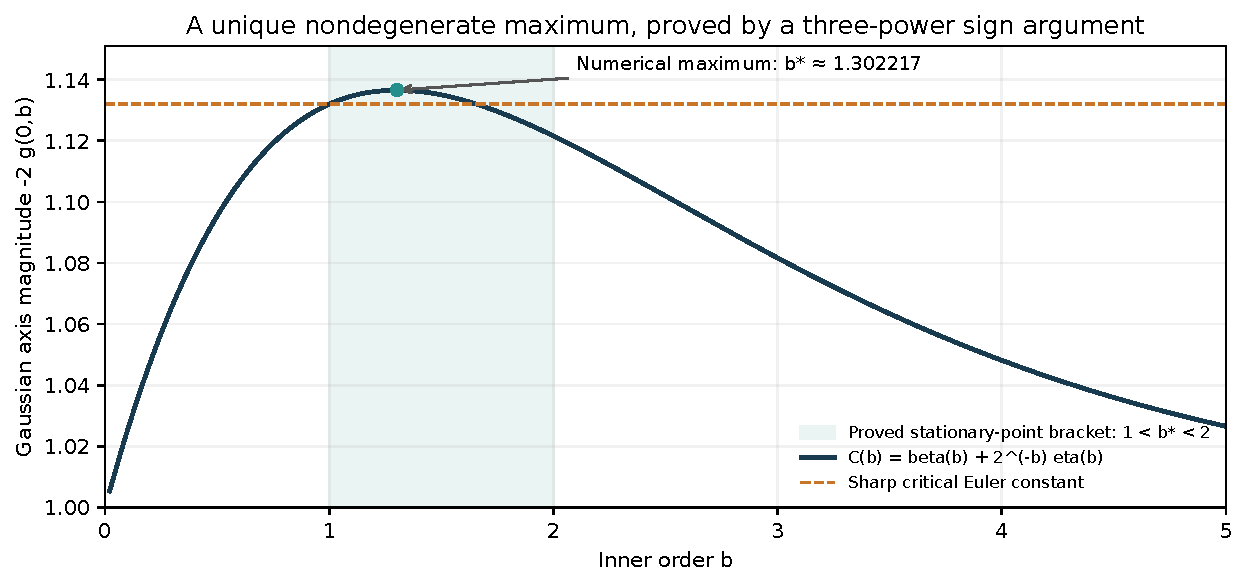
\includegraphics[width=\textwidth]{figures/Gaussian_axis_maximum.pdf}
\caption{Numerical values of the exact Gaussian axis expression and its
stationary-point marker. The shaded interval is the proved bracket for
the unique maximum; the horizontal line is the proved sharp critical
Euler constant. The maximum's displayed decimal location is diagnostic.
The larger global Gaussian maximum does not supply a universal Euler
constant in arbitrary supercritical parameter regions.}
\label{subpick:fig:Gaussian-axis}
\end{figure}
